\RequirePackage[l2tabu, orthodox]{nag}
\documentclass[11pt,uplatex,a4paper]{jsarticle}
%% file: fem2dp-2.tex
%% author: Junichi Motohisa
%% created: 2017-11-21 18:32:34
%% last saved : Time-stamp: <Tue Aug 29 18:06:24 JST 2023>
\usepackage[dvipdfmx]{graphicx}
\usepackage{multicol}
\usepackage{cite}
%\usepackage{mathptmx}
%\usepackage{color}
\usepackage{lscape}
% \usepackage{dcolumn}
\usepackage{moreverb}
% \usepackage[a4paper,margin=1in]{geometry}
\usepackage[driver=dvipdfmx,truedimen]{geometry}
% \geometry{left=30truemm,right=25truemm,top=25truemm,bottom=25truemm}
\geometry{margin=1truein}
% \usepackage[a4paper,margin=1in]{geometry}

%% taken from https://github.com/ryseto/emacs_and_tex/blob/master/template.tex
%% begin
\usepackage{amsmath,amsfonts,amsthm}
\usepackage{bm}
\usepackage[protrusion=true,expansion=true]{microtype}
\usepackage{siunitx}
\usepackage{xcolor}
%\usepackage[pdftex]{graphicx}
%\usepackage[pdftex,bookmarks,colorlinks]{hyperref}
% \usepackage[dvipdfmx]{hyperref}
% \usepackage{pxjahyper}
\usepackage[english]{babel}
\usepackage[T1]{fontenc}
\usepackage[utf8]{inputenc}
\usepackage{newtxtext}
\usepackage[varg]{newtxmath}
\usepackage{booktabs}
\usepackage{datetime}
\usepackage{setspace}
\usepackage{enumitem}
\usepackage{cleveref}
\usepackage[numbers]{natbib}

% \bibliographystyle{abbrvnat}
\setlist{itemsep=-3pt}
%% end

\def\d#1#2{\frac{d #1}{d #2}}
\def\dd#1#2{\frac{d^2 #1}{d #2^2}}
\def\pd#1#2{\frac{\partial #1}{\partial #2}}
\def\pdd#1#2{\frac{\partial^2 #1}{\partial #2^2}}
\def\Ene{\varepsilon}
\def\DOS{\mathcal{D}}
\def\vec#1{{\bm{#1}}}
\def\kvec{\bm{k}}
\def\kvecp{{\bm{k}'}}
\def\subvec#1{{\boldsymbol{\small #1}}}
 
\def\GP{{\vec{G}_\parallel}}
\def\GPP{{\vec{G}^\prime_\parallel}}
\def\KP{{\vec{k}_\parallel}}
\def\KP{{\vec{k}_\parallel}}
\def\XP{{\vec{x}_\parallel}}

\def\EneK{\varepsilon_{\kvec}}
\def\EneKp{\varepsilon_{\kvec^{'}}}
\def\EneKn{\varepsilon_{\kvec n}}
\def\EneKnp{\varepsilon_{\kvec^{'} n^{'}}}
\def\EneKm{\varepsilon_{m \vec{k}}}
\def\EneKmp{\varepsilon_{m' \vec{k}'}}

\def\bra#1{{\langle #1 |}}
\def\ket#1{{| #1 \rangle}}
\def\braket#1#2{{\langle #1 | #2 \rangle}}
\def\av#1{{\langle #1 \rangle}}

\def\sinc{\mathrm{sinc}}
\def\sgn{\mathrm{sgn}_{n,p}}
\def\Tr{{\mathrm{Tr}\, }}

\def\micon{\mathrm{\mu m}}
\def\nm{\mathrm{nm}}

\begin{document}

\title{Title}
\author{J.~Motohisa\\Graduate School of IST, Hokkaido University}
\date{\shortdate\today \, \ampmtime }
\maketitle

\section{Introduction}

\section{Ballistic FET in 2D}
\subsection{Top of the barrier}
Top of the barrierの位置を定める式は
\begin{equation}
 E_0 = -q(\alpha_G V_G + \alpha_D V_D + \alpha_S V_S) + \frac{q^2}{C_{\Sigma}} n_s
  \label{eqn:tob2D1}
\end{equation}
ここで
\begin{equation}
 n_s = \frac{\mathcal{D}_{2D}k_B T}{2}
  \left[
   F_0(\frac{E_F - E_0}{k_B T})+
   F_0(\frac{E_F -q V_D- E_0}{k_B T})
										 \right]
  \label{eqn:2degdens}
\end{equation}
であり、ここで$F_j(\eta)$は第$j$次のフェルミ--ディラック積分、$\mathcal{D}_{2D}$は2次元電子の状態密度
\begin{equation}
 \mathcal{D}_{2D} = \frac{m^*_{DOS}}{\pi \hbar^2}
\end{equation}
また
\begin{equation}
 \alpha_{G} = \frac{C_G}{C_{\Sigma}}, \quad
  \alpha_{D} = \frac{C_D}{C_{\Sigma}}, \quad
   \alpha_{S} = \frac{C_S}{C_{\Sigma}}, \quad
\end{equation}
および
\begin{equation}
 C_{\Sigma} = C_{G} + C_{D} + C_{S}
\end{equation}
である。\footnote{ここで$C_S$はソース--チャネル間との容量であり、半導体容量ではない。}
ここで$V_{G}=V_{GS}+V_{S}$、$V_{D}=V_{DS}+V_{S}$とおくと式(\ref{eqn:tob2D1})は
$\alpha_G + \alpha_D + \alpha_S =1$を使って
\begin{equation}
 E_0 + q V_S = -q(\alpha_G V_{GS} + \alpha_D V_{DS}) + \frac{q^2}{C_{\Sigma}} n_s
\end{equation}
この左辺を$E'_0$とおいて、$E_0 = E'_0 - q V_{S}$を式(\ref{eqn:2degdens})に代入すると
\begin{equation}
 n_s = \frac{\mathcal{D}_{2D}k_B T}{2}
  \left[
   F_0(\frac{E_F + q V_S - E'_0}{k_B T})+
   F_0(\frac{E_F + q V_S - q V_D- E'_0}{k_B T})
									 \right]
\end{equation}
よって$E_{Fs}=E_F+ q V_S$とおいて$E'_0$をあらためて$E_0$と置けば
\begin{equation}
 E_0 = -q(\alpha_G V_{GS} + \alpha_D V_{DS}) + \frac{q^2}{C_{\Sigma}} n_s
\end{equation}
ならびに
\begin{equation}
 n_s = \frac{\mathcal{D}_{2D}k_B T}{2}
  \left[
   F_0(\frac{E_{Fs} - E_0}{k_B T})+
   F_0(\frac{E_{Fs} - q V_D- E_0}{k_B T})
									 \right]
\end{equation}
がTop of the barrier を求める際に解くべき式となる。
この時点でパラメータは$C_{G} (=C_{OX}), C_{D}, C_{S}, E_{Fs}$もしくは
$\alpha_{G}, \alpha_{D}, C_{\Sigma}, E_{Fs}$
の組に集約される。



Top of the Barrierのエネルギー$E_0$は
\begin{equation}
 E_0 + \alpha_D q V_{DS} + \alpha_G q V_{GS} -
  q^2\frac{n_{2D}(E_F - E_0)+n_{2D}(E_F-E_0-qV_{DS})}{2 C_{eff}}=0
  \label{eqn:tob}
\end{equation}
を解くことによって求めることができる。
ここで
\begin{equation}
 n_{2D}(E) = \mathcal{D}_{2D}k_B T \ln (1+\exp(\frac{E}{k_B T}))
\end{equation}
であり、また$\mathcal{D}_{2D}$は2次元の状態密度であり$\mathcal{D}_{2D}=m^*/\pi \hbar^2$である。

  \subsection{近似}
式(\ref{eqn:tob})を近似すると
\begin{equation}
 E_0 + \alpha_D q V_{DS} + \alpha_G q V_{GS} -
  q^2\frac{\mathcal{D}_{2D}(E_F - E_0)+\mathcal{D}_{2D}(E_F-E_0-qV_{DS})}{2 C_{eff}}=0
\end{equation}
と書ける。
 この式を解くと
 \begin{equation}
  \frac{E_0}{q} = -\frac{\alpha_G V_{GS} + \alpha_D V_{DS}}{1+C}
   + \frac{C}{1+C} (\frac{E_{F}}{q}-\frac{V_{DS}}{2})
 \end{equation}
 ここで
\begin{equation}
 C=\frac{q^2}{C_{eff}}\mathcal{D}_{2D} = \frac{q^2m^*}{C_{eff}\pi \hbar^2}
\end{equation}
である。
さらに実際top of the barrierにおける電子密度$N_{2D}$は
\begin{equation}
 \begin{split}
 N_{2D} &= \frac{1}{2}
  (n_{2D}(E_F-E_0) + n_{2D}(E_F-E_0-qV_{DS})) \\
  &\sim \frac{C C_{eff}}{q} (\frac{E_F - E_0}{q} - \frac{V_{DS}}{2}) \\
  &\propto \frac{1}{q}\frac{C}{1+C} \alpha_G C_{eff} V_{GS}
  = \frac{1}{q}\frac{1}{1+1/C} \alpha_G C_{eff} V_{GS}
 \end{split}
\end{equation}
これらの式から、有効質量$m^*$が大きくなった場合、
状態密度の増大によるキャリア密度の増大効果と、
Top of the barrierのエネルギー$E_0$の低下量が小さくなる効果がほぼ総裁し、
電流は増加する可能性があるものmerginal な増加であり、
実際には、injection velocityが低下すると考えられるため、
電流が減少すると予想される。

% $V_{GS}$ top of the barrier $E_0$の
% $V_{GS}$の増加に対する
% このため$V_{GS}$に対する電流の増加は小さくなることがわかる。

\subsection{Model of Ballistic One-dimensional Transistor} % \cite{motohisa}}}} 
Next\footnote{This section is taken from \protect{\cite{motohisa}}},
brief outline to calculate drain current in ballistic NW-FETs is described following the
model of ballistic transistor by Lundstrom and co-workers\cite{LG,Rahman:2003ug}. 
The electron density in one-dimensional (1D) electron system is calculated as
%\begin{equation}
\begin{align}
 n_{\mathrm{1D}} &= \int_{E_C}^\infty \frac{\sqrt{2 m^*}}{\pi \hbar}\frac{1}{\sqrt{E-E_{C}}}  \frac{1}{1+\exp\left(\frac{E - E_F}{k_B T}\right)} dE \\
 &= \mathcal{D}_{\mathrm{1D}} F_{-1/2}\left( \frac{E_F-E_C}{k_B T}
 \right) \ ,
 \label{eqn:1deg0}
\end{align}
%\end{equation}
where $E_F$ is the Fermi level,
$E_C$ represents the bottom of the conduction band, $m^*$ is the density-of-state effective mass,
$\mathcal{D}_{\mathrm{1D}}$ is the effective density of state in 1D system given by
\begin{equation}
 \mathcal{D}_{\mathrm{1D}} = \frac{\sqrt{2 m^* k_B T}}{\sqrt{\pi} \hbar} \ , 
\end{equation}
$F_j(\eta)$ is a Fermi-Dirac integral of the $j$-th order
\begin{equation}
 F_{j}(\eta) = \frac{1}{\Gamma(j+1)} \int_0^\infty \frac{\eta_0^j}{1+\exp(\eta_0-\eta)} d \eta_0 \ , 
\end{equation}
and $\Gamma(z)$ is the Gamma function.
Drain current of the transistor in the ballistic regime is determined by the net carrier flow
from source to drain with energy larger than the top of the barrier $U_{\mathrm{SCF}}$, shown in Fig. \ref{fig:TOB}.  
$U_{\mathrm{SCF}}$ is determined in a self-consistent way by solving the following equation:
\begin{equation}
 U_{\mathrm{SCF}} = -q(\alpha_{\mathrm{G}} V_{\mathrm{G}} + \alpha_{\mathrm{D}} V_{\mathrm{D}} + \alpha_{\mathrm{S}} V_{\mathrm{S}}) + \frac{q^2}{C_{\Sigma}} n_s
  \label{eqn:tob1D1}
\end{equation}
Here $n_s$ represents the electron density at the top of the barrier and given by the sum of the contribution from the
source side and the drain side.
Thus, using Eq. (\ref{eqn:1deg0}), $n_s$ in 1D system is given by
\begin{equation}
 n_s = \frac{\mathcal{D}_{\mathrm{1D}}}{2}
  \left[
   F_{-1/2}(\frac{E_F - U_{\mathrm{SCF}}}{k_B T})+
   F_{-1/2}(\frac{E_F -q V_{\mathrm{D}}- U_{\mathrm{SCF}}}{k_B T})
										 \right]
  \label{eqn:1degdens}
\end{equation}
% where and
% $\mathcal{D}_{\mathrm{1D}}$ is an effective density of states of one-dimensional electron gas
% \begin{equation}
%  \mathcal{D}_{\mathrm{1D}} = \frac{m^*_{DOS}}{\pi \hbar^2}
% \end{equation}
Furthermore, $V_i$'s ($i=\mathrm{G}$, $\mathrm{D}$, or $\mathrm{S}$) are the
voltage at the terminals of FETs, 
$\alpha_i$'s are the leverage factor of each terminals and given by the capacitance $C_{i}$ associated with the each terminals as
\begin{equation}
 \alpha_{G} = \frac{C_{\mathrm{G}}}{C_{\Sigma}}, \quad
  \alpha_{\mathrm{D}} = \frac{C_{\mathrm{D}}}{C_{\Sigma}}, \quad
   \alpha_{\mathrm{S}} = \frac{C_{\mathrm{S}}}{C_{\Sigma}}, \quad
\end{equation}
and
\begin{equation}
 C_{\Sigma} = C_{G} + C_{\mathrm{D}} + C_{\mathrm{S}}
\end{equation}
The values of these capacitors are set so that to fit with are used to fit the experimental data of $S$ and DIBL, 
as described in Refs. \cite{Rahman:2003ug,Liang:2007uh}.
By setting $V_{G}=V_{\mathrm{GS}}+V_{\mathrm{S}}$、$V_{\mathrm{D}}=V_{\mathrm{DS}}+V_{\mathrm{S}}$, Eq. (\ref{eqn:tob1D1}) reduces to
\begin{equation}
 U_{UCF} + q V_{\mathrm{S}} = -q(\alpha_{\mathrm{G}} V_{\mathrm{GS}} + \alpha_{\mathrm{D}} V_{\mathrm{DS}}) + \frac{q^2}{C_{\Sigma}} n_s
\end{equation}
using $\alpha_{\mathrm{G}} + \alpha_{\mathrm{D}} + \alpha_{\mathrm{S}} =1$. 
By replacing $U_{\mathrm{SCF}} = E_0 - q V_{\mathrm{S}}$ and $E_F =E_{\mathrm{Fs}}-  q V_{\mathrm{S}}$ , 
% we obtain
% \begin{equation}
%  n_s = \mathcal{D}_{\mathrm{1D}}
%   \left[
%    F_{-1/2}(\frac{E_F + q V_{\mathrm{S}} - U'_{SCF}}{k_B T})+
%    F_{-1/2}(\frac{E_F + q V_{\mathrm{S}} - q V_{\mathrm{D}}- U'_{SCF}}{k_B T})
% 									 \right]
% \end{equation}
% By setting  and rewriting $U'_{SCF}$ as $U_{\mathrm{SCF}}$, we obtain
\begin{equation}
 E_{0} = -q(\alpha_{\mathrm{G}} V_{\mathrm{GS}} + \alpha_{\mathrm{D}} V_{\mathrm{DS}}) + \frac{q^2}{C_{\Sigma}} n_s
  \label{eqn:TOB}
\end{equation}
and
\begin{equation}
 n_s = \mathcal{D}_{\mathrm{1D}}
  \left[
   F_{-1/2}(\frac{E_{\mathrm{Fs}} - E_0}{k_B T})+
   F_{-1/2}(\frac{E_{\mathrm{Fs}} - q V_{\mathrm{DS}}- E_0}{k_B T})
												   \right]
  \label{eqn:1deg}
\end{equation}
Equation (\ref{eqn:TOB}) is identical to Eq. (30) in Ref. \cite{Lind}, or
Eq. (35) in \cite{Yu:2008tv}, except for that multiple subbands and
nonparabolicity are not considered in $n_s$ given in Eq. (\ref{eqn:1deg}).
The drain current $I_{\mathrm{DS}}$ is calculated as \cite{Lind,LG,Yu:2008tv}
%\begin{equation}
\begin{align}
 I_{\mathrm{DS}} &=   \frac{2q k_B T}{h}
  \left[
   F_0\left((E_{\mathrm{Fs}}-E_{0})/k_B T\right)
-  F_0\left((E_{\mathrm{Fs}}-E_{0}-qV_{\mathrm{DS}})/k_B T\right)
							   \right] \\
&=  \frac{2q k_B T}{h}
  \left[\ln \left(1+ \exp \left(\frac{E_{\mathrm{Fs}}-E_{0}}{k_B T}\right)\right)
 -\ln \left(1+ \exp \left(\frac{E_{\mathrm{Fs}}-E_{0}-qV_{\mathrm{DS}}}{k_B T} \right)
 \right)
 \right]
 \label{eqn:IDSballistic}
\end{align}
% \end{equation}
If one has to take into account multiple subbands in NWs,
it is doable by considering quantized energy $E_n$ 
and taking sum of the contribution from each subbands for $n_s$ (Eq. (\ref{eqn:1deg}))
and $I_{\mathrm{DS}}$ (Eq. (\ref{eqn:IDSballistic})), as described in Refs. \cite{Lind,Yu:2008tv}.

\begin{figure}[htbp]
 \centering
 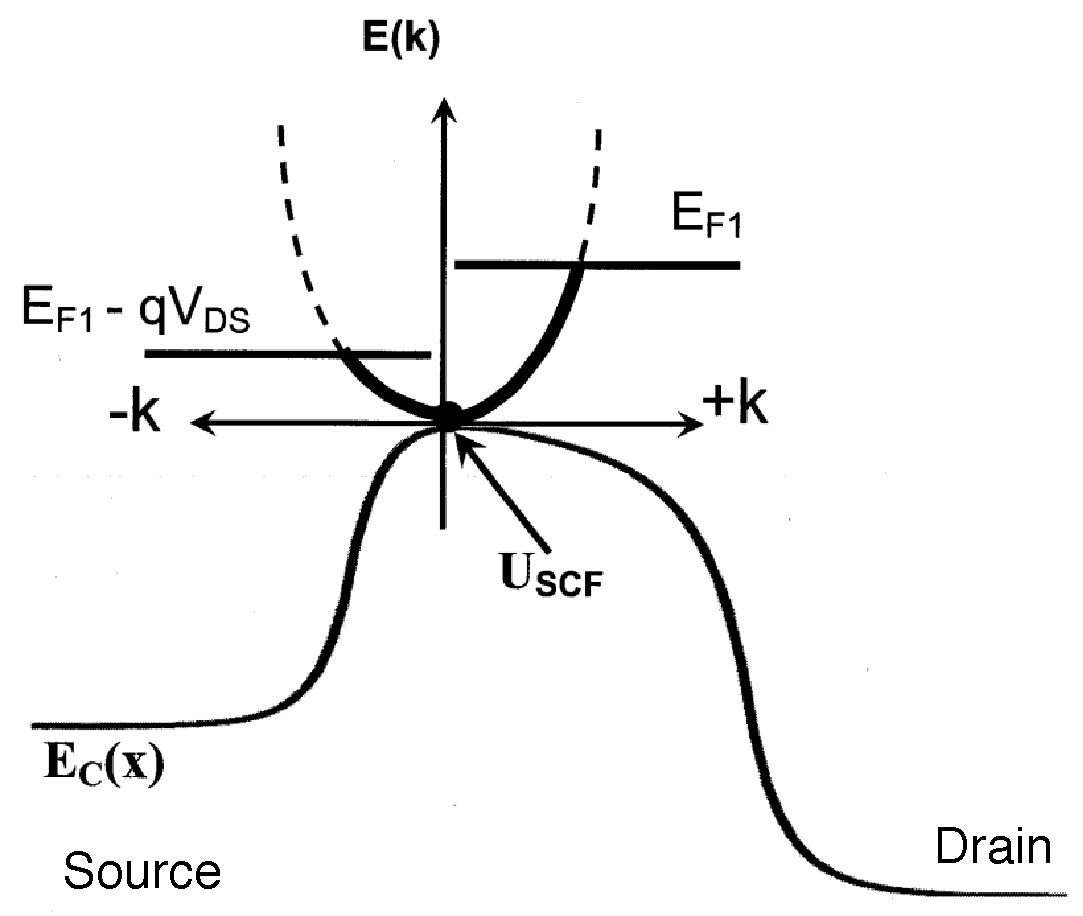
\includegraphics[keepaspectratio,width=8cm,bb=0 0 520 439]{TOB.pdf}
 \caption{Illustration to show how the top of the barrier is determined by the Fermi level in the
 drain and source.
 The carriers (electrons) from source to drain (or vice versa) has positive (negative) wavevector $k$ and contribute to the
 positive drain current $I_{\mathrm{DS}}$, and total carrier density at the
 top of the barrier is determined by the some of the carriers from source and drain.
% Reproduced and modified with permission from Ref. \protect{\cite{Rahman:2003ug}}.
 Copyright @ IEEE. All rights reserved. Reprinted, with permission, from Ref. \protect{\cite{Rahman:2003ug}}.
 % Copyright IEEE.
 \label{fig:TOB}}
\end{figure}

\appendix
\section{Notes on band nonparablicity}
2バンドモデルでは\cite{mikoshiba}
\begin{equation}
 \frac{m^*}{m_0} = \frac{E_G}{E_P+E_G} = \frac{1}{1+E_P/E_G}
\end{equation}
および
\begin{equation}
 \frac{\hbar^2k^2}{2m^*} \sim
  E \left[ 1 + \frac{E_p^2}{E_G(E_G+E_p)^2}E + \cdots
	\right]
\end{equation}
となる。ここで$E_P$はKaneのパラメータである。
\begin{equation}
 E_P = \frac{4 m_0}{3 \hbar^2}|P|^2
\end{equation}
\begin{equation}
 P=-i\frac{i\hbar^2}{m_0}\langle x | p_x| X\rangle
\end{equation}
である。
これより
\begin{equation}
 \alpha = \frac{E_P^2}{E_G(E_G+E_p)^2} = \frac{1}{E_G}(1+\frac{E_G}{E_P})^{-2}
\end{equation}
となる。
また、
\begin{equation}
 \frac{E_P}{E_G} = \frac{m_0}{m^*}-1
\end{equation}
となるから
\begin{equation}
 \alpha = \frac{1}{E_G} (1+\frac{1}{m_0/m^*-1})^{-2}
  = \frac{1}{E_G} (1-\frac{m^*}{m_0})^2
\end{equation}

ところで\cite{Vurgaftman}では
\begin{equation}
 E_{P,V}=\frac{2\hbar^2}{m_0}|P|^2
\end{equation}
となっているので
\begin{equation}
 E_P =\frac{2}{3}E_{P,V}
\end{equation}
である。よって
\begin{equation}
 \frac{m^*}{m_0} =  \frac{1}{1+2E_{P,V}/3E_G}
\end{equation}

実効的なサブバンド有効質量はエネルギーとともに増加し、
実効的な非サブバンド非放物線性はエネルギーとともに減少する

The effective sub-band mass increases with energy, and the effective non-parabolicity factor decreases

\section{Density of States}
3次元において状態密度は
\begin{equation}
\mathcal{D}_{3D}(E) = \frac{2}{(2 \pi)^3} \int \frac{dS_{E(k)}}{\nabla_k E(k)}
\end{equation}
により計算される\cite{kittel}。積分は等エネルギー面上で行う。同様に2次元では
\begin{equation}
\mathcal{D}_{2D}(E) = \frac{2}{(2 \pi)^2} \int \frac{ds_{E(k)}}{\nabla_k E(k)}
\end{equation}
で積分を等エネルギー線上で行い、さらに1次元では
\begin{equation}
 \mathcal{D}_{1D}(E) = \frac{2}{2 \pi} [
  (\d{E}{k})^{-1}|_{E(k)}
  +(\d{E}{k})^{-1}|_{E(-k)}
  ]
\end{equation}
となる。

1次元の場合に
\begin{equation}
 E(1+\alpha E) = \frac{\hbar^2 k^2}{2 m^*}\equiv \Ene_k
  \label{eqn:dispersion}
\end{equation}
として計算してみる。式(\ref{eqn:dispersion})より
\begin{equation}
 E=\frac{\sqrt{1+4\alpha \Ene_k}-1}{2\alpha}
\end{equation}
であるから
\begin{equation}
 \d{E}{k} = \frac{1}{2\alpha 2 \sqrt{1+4\alpha \Ene_k}} 4 \alpha \frac{\hbar^2 k }{m^*} =
  \frac{\hbar^2}{m^*} \frac{k}{\sqrt{1+4\alpha \Ene_k}}
  = \frac{\hbar^2}{m^*} \frac{k}{1+2\alpha E}
\end{equation}
となる。\footnote{式(\protect{\ref{eqn:dispersion}})を直接微分しても得られる。}
よって
\begin{subequations}
\begin{align}
 \mathcal{D}_{1D}(E)
 &= \frac{1}{\pi}((\d{E}{k})^{-1}) \times 2 \\
 & = \frac{2}{\pi} \frac{m^*}{\hbar^2} \frac{1+2\alpha E}{\sqrt{2 m^* E(1+\alpha E)}/\hbar} \\
 &= \frac{\sqrt{2 m^*}}{\pi \hbar} 
 \frac{1+2 \alpha E}{\sqrt{E(1+\alpha E)}}
 \end{align}
\end{subequations}
これは\cite{Godoy}や\cite{Lind}の式と同じとなる。

2次元では
\begin{subequations}
\begin{align}
 \mathcal{D}_{2D}(E)
 & = \frac{1}{2\pi^2}((\d{E}{k})^{-1}) \times 2 \pi k \\
 & = \frac{m^*}{\pi\hbar^2} (1+2 \alpha E)
\end{align}
\end{subequations}
となる。

\begin{thebibliography}{99}
  \bibitem{LG} Lundostrom and Gao Ballistic Nanotransistors
  \bibitem{Lind} Lind, E. (2016). High frequency III{\textendash}V nanowire MOSFETs. Semiconductor Science and Technology, 31(9), 93005–93014. https://doi.org/10.1088/0268-1242/31/9/093005
  \bibitem{mikoshiba} 御子柴 半導体の物理
  \bibitem{Vurgaftman} Vurgaftman
  \bibitem{kittel} C. Kittel, 固体物理学入門
  \bibitem{Godoy} Andr\'es Godoy, Zhicheng Yang, Umberto Ravaioli, Francisco Gámiz. (2005) Effects of nonparabolic bands in quantum wires. Journal of Applied Physics 98:1, 013702.
 \bibitem{motohisa} J. Motohosia and S. Hara, \textit{Nanowire Field Effect Transistor},
	 in {\em Fundamental Properties of Semiconductor
  Nanowires\/} Fukata N and Rurali R (eds) 2021, (Singapore: Springer Singapore).
\bibitem{Yu:2008tv}
B.~Yu, L.~Wang, Y.~Yuan, P.M. Asbeck, Y.~Taur, IEEE Transactions on Electron
  Devices \textbf{55}(11), 2846 (2008)
\bibitem{Liang:2007uh}
G.~Liang, J.~Xiang, N.~Kharche, G.~Klimeck, C.M. Lieber, M.~Lundstrom, Nano
  Letters \textbf{7}(3), 642 (2007)
\bibitem{Rahman:2003ug}
A.~Rahman, {Jing Guo}, S.~Datta, M.~Lundstrom, IEEE Transactions on Electron
  Devices \textbf{50}(9), 1853 (2003)

\end{thebibliography}
%% \bibliography{/Users/motohisa/Dropbox/Papers/rse}

\end{document}

